
% !TeX root = first.tex

\section{Grundlagen des Personalmanagements} 
\label{sec:grundlagenpersonalmanagement}

\subsection{Definition, Bedeutung und Ziele, Historie}
\label{sec:gl_definition}
Das Personalmanagement umfasst alle organisatorischen und administrativen Tätigkeiten, die sich auf die Planung, Entwicklung, Führung und Kontrolle der Mitarbeiter eines Unternehmens oder einer Organisation beziehen. Das Personalmanagement beinhaltet die Gestaltung von Personalstrategien, -richtlinien und -prozessen. Dabei liegt die entscheidende Funktion des Personalmanagements darin, die richtigen Personen mit den erforderlichen Fähigkeiten und Qualifikationen am richtigen Ort und zur richtigen Zeit zur Verfügung zu stellen. Des Weiteren ist das Personalmanagement für die Personalentwicklung, die Mitarbeitermotivation, die Leistungsbeurteilung, die Vergütung, die Arbeitsbedingungen, die Mitarbeiterbindung und das Konfliktmanagement verantwortlich. Das wesentliche Ziel des Personalmanagements ist es, eine positive und produktive Arbeitsumgebung zu schaffen, in der sich die Mitarbeiterinnen und Mitarbeiter wertgeschätzt, motiviert und gefördert fühlen und somit zu dem langfristigen Erfolg und der Wettbewerbsfähigkeit eines Unternehmens beitragen.\footnote{Vgl. \cite{personio:PersoManagement}}

Das Personal, beziehungsweise der Mensch, ist die wertvollste Ressource und somit auch zentrales Kapital eines Unternehmens. Durch talentierte und hochqualifizierte Mitarbeiter werden Wettbewerbsvorteile gegenüber Marktkonkurrenten geschaffen. Das Personalmanagement spielt die Schlüsselrolle bei der Rekrutierung und Bindung dieser Talente. Mit effektive Personalmanagementpraktiken und einer positiven Unternehmenskultur können die Produktivität und Leistung der Mitarbeiter gefördert werden und eine Arbeitsatmosphäre entstehen, in der sich die Mitarbeiter wertgeschätzt, motiviert und engagiert fühlen. Zu dem ist das Personalmanagement für die Risikominimierung von rechtlichen Problemen und Konflikten, indem es Richtlinien und Verfahren zur Einhaltung von Arbeitsgesetzten und -vorschriften implementiert.\footnote{Vgl. \cite{lernort-mint:PMBedeutungZiele}}

%Versuch der Vektorgrafik
%\begin{figure}
%\centering
%\def\svgwidth{375pt}
%\input{bilder/PMHistorie.pdf_tex}
%\caption{Historische Entwicklung des Personalmanagements}
%\label{fig:PMHistorie}
%\end{figure}

\begin{figure}%[htb]
\centering
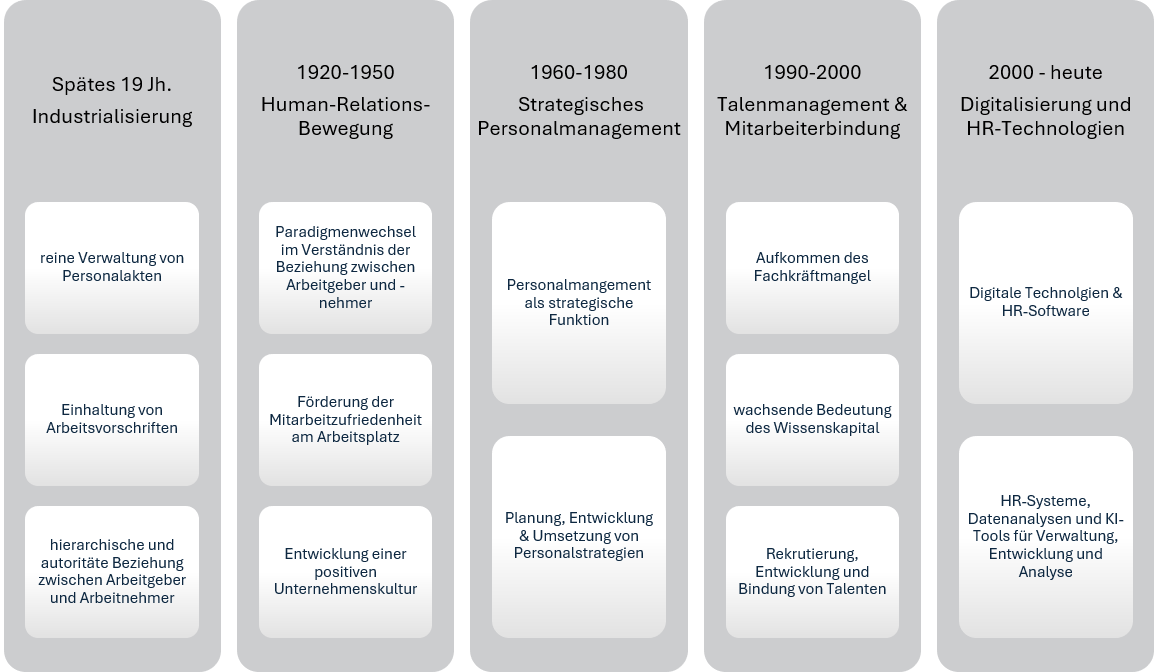
\includegraphics[scale=0.5]{pmhistorie}
\caption{Historische Entwicklung des Personalmanagements}
\label{fig:pmhistorie}
\end{figure}

In der Abbildung~\ref{fig:pmhistorie} wird die Historische Entwicklung des Personalmangements dargestellt.\footnote{Vgl. \cite{Haufe2016}}

 \begin{description}
\item[Spätes 19. Jahrhundert:] Autoritärer Führungsstil mit Unterdrückung des Personals. Das Personalmanagement bestand aus der Verwaltung von Personalakten und Einhaltung von Arbeitsvorschriften.

\item[1920-1950:] Entstehung eines neuen Paradigmas im Verständnis der Beziehung zwischen Arbeitgeber und -nehmer. Die Mitarbeiterzufriedenheit wurde gefördert und eine positive Unternehmenskultur geschaffen.

\item[1960-1980:] Einführung eines strategischen Personalmanagements als Funktion für die Planung, Entwicklung \& Umsetzung der Personalstrategien.

\item[1990-2000:] Durch den Fachkräftemangel wuchs die Bedeutung von Wissenskapital. Es wurden Konzepte für die Rekrutierung, Entwicklung und Bindung von Talenten erstellt.

\item[2000-heute:] Die Digitalisierung sowie die daraus resultierenden HR Technologien erweitern die Bandbreite des Personalmanagements.

\end{description}

\subsection{Personalplanung}
Die Personalplanung ist ein zentrales Element des Personalmanagements und bezieht sich auf den systematischen Prozess der vorausschauenden und bedarfsorientierten Planung aller personellen Ressourcen eines Unternehmens. Die Personalplanung ist ein kontinuierlicher und systematischer Prozess innerhalb des Personalmanagements, der darauf abzielt, den optimalen Einsatz der menschlichen Ressourcen in einem Unternehmen sicherzustellen. Die Personalplanung umfasst nicht nur die Planung, sondern auch die Analyse und Prognose des aktuellen und zukünftigen Personalbedarfs. Dabei werden die internen und externen Faktoren wie die Unternehmensstrategien, Marktbedingungen und gesetzliche Rahmenbedingung berücksichtigt.\footnote{Vgl. \cite[S. 2-11]{Jahn03:EntwicklungPM}}

\begin{figure}%[htb]
\centering
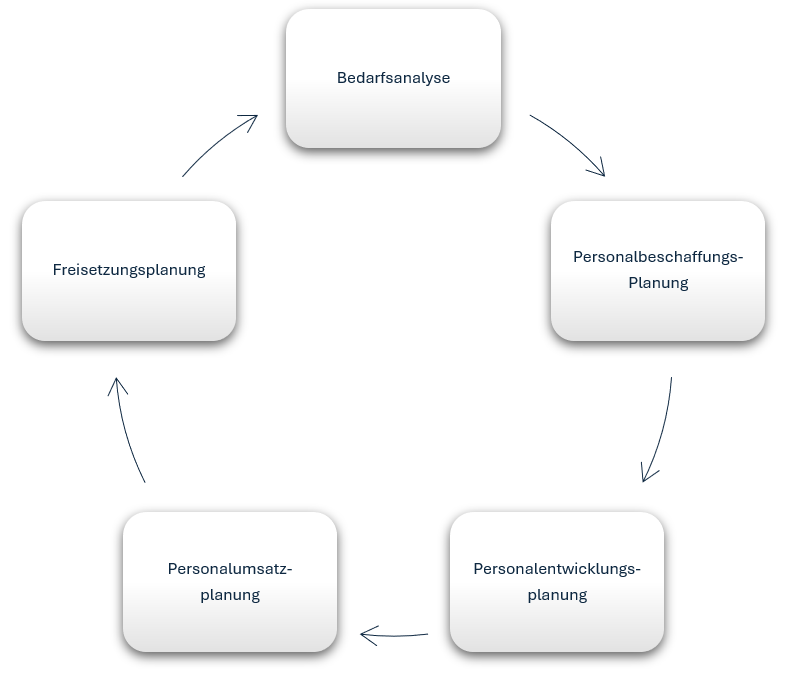
\includegraphics[scale=0.4]{personalplanungsprozess}
\caption{Personalplanungsprozess}
\label{fig:personalplanungsprozess}
\end{figure}

Die Abbildung~\ref{fig:personalplanungsprozess} beschreibt den Prozesszyklus der Personalplanung. In der Bedarfsanalyse wird der aktuelle und zukünftige Personalbedarf anhand von Geschäftszielen, Arbeitsaufgaben und Projekten ermittelt. Dabei werden die benötigten Kompetenzen und Fähigkeiten analysiert, um die Unternehmensziele zu erreichen. In der Personalbeschaffungsplanung wird auf Basis der Bedarfsanalyse die Strategien und Maßnahmen zur Rekrutierung neuer Mitarbeiterinnen und Mitarbeiter entwickelt. Solcher Maßnahmen sind beispielsweise interne Förderung, externe Rekrutierung oder das Einsetzen von Zeitarbeitskräften sein. In der Personalumsatzplanung werden Maßnahmen zur Mitarbeiterbindung und -motivation entwickelt, um die Fluktuation zu reduzieren und die Bindung von Talenten an das Unternehmen zu fördern. Die Controlling- und Anpassungsphase überwacht und bewertet die Ergebnisse der Personalplanungsmaßnahmen, damit der Erfolg der Maßnahmen bemessen werden kann, bei Bedarf Anpassungen vorgenommen werden können und auf Veränderungen in der Unternehmensumgebung oder unerwartete Entwicklungen reagieren zu können.\footnote{Vgl. \cite{bwllexikon2024}}

\subsection{Personalbeschaffung}
\label{sec:personalbeschaffung} %Bezug
Die Personalbeschaffung ist ein essenzieller Teil der Personalwirtschaft, der darauf abzielt, den Personalbedarf eines Unternehmens zu decken. Dies umfasst die Suche nach qualifizierten Mitarbeitern in Bezug auf Quantität, Qualität, Standort und Zeitrahmen. Die Planung, Suche und Einstellung neuer Mitarbeiter sollte kosteneffizient erfolgen. Der Prozess besteht aus der Personalplanung, Auswahl der Beschaffungswege, Personalauswahl und Onboarding. Interne Beschaffung nutzt vorhandenes Personal und ist kostengünstig, während externe Beschaffung Bewerber von außen anzieht. Aktive Beschaffung erfolgt proaktiv durch Anzeigen und Anreize, passive Beschaffung durch Initiativbewerbungen. Die Auswahl erfolgt anhand objektiver Kriterien wie Gehalt und Referenzen, oft mittels Vorstellungsgespräche und Assessment-Centern. Die passive Variante, die auf Initiativ- und Blindbewerbungen abzielt, involviert Bewerber, die sich unaufgefordert dem Unternehmen anbieten, oft aufgrund des guten Rufs des Unternehmens. Zielgerichtete Employer Branding Maßnahmen unterstützen das Unternehmen dabei, sich als attraktiven Arbeitgeber zu positionieren. Vorteile dieser Herangehensweise sind eine breite Auswahl an potenziellen Kandidaten, die Einführung neuer Kenntnisse und Ideen ins Unternehmen, sowie das Ausbleiben interner Fort- und Weiterbildungskosten. Zudem ermöglicht sie ein kritisches Hinterfragen der bestehenden Prozesse. Jedoch sind auch Nachteile zu berücksichtigen. Dazu zählen höhere Kosten für das Recruiting, eine deutlich erhöhte Gefahr von Fehlbesetzungen, potenzielle Enttäuschung unter internen Mitarbeitern, die möglicherweise für die Stelle geeignet gewesen wären, sowie längere Einarbeitungszeiten. Bei der Auswahl der Bewerber werden verschiedene Kriterien berücksichtigt, wie etwa die Gehaltsvorstellungen der Bewerber, ihre Referenzen und ihr Auftreten. Der Auswahlprozess soll stets objektiv, zuverlässig und fair sein, um jedem Bewerber gleiche Chancen zu bieten. Zunächst werden die Bewerbungen gründlich geprüft und analysiert, bevor Vorstellungsgespräche angesetzt und durchgeführt werden. Schließlich entscheidet das Unternehmen, welcher Bewerber die Anforderungen am besten erfüllt. Ein wichtiges Instrument der Personalauswahl ist das Assessment-Center, das in jüngster Zeit an Bedeutung gewonnen hat. Es dient der standardisierten Bewertung mehrerer Bewerber und zielt darauf ab, deren Analysefähigkeiten, Auffassungsgabe und andere Fähigkeiten zu ermitteln. Im Assessment-Center werden in der Regel verschiedene Tests mit den Bewerbern durchgeführt.\footnote{Vgl. \cite{Studyflix2024}} 


\subsection{Personalentwicklung}
Die Förderung und Entwicklung von Talenten wird für Unternehmen zunehmend wichtiger. Der sich wandelnde Arbeitsmarkt und die ständig verkürzte Lebensdauer von Wissen erfordern eine verstärkte Initiative seitens der Arbeitgeber, die Fähigkeiten ihrer Mitarbeiter zu erweitern. Auch der technologische und organisatorische Wandel erfordert kontinuierliches Lernen. Die Unterstützung der Mitarbeiter bei ihrer beruflichen und persönlichen Entwicklung trägt außerdem dazu bei, Schlüsselpersonen langfristig an das Unternehmen zu binden und die Leistungsstärke sowie Kernkompetenzen zu stärken. Die Personalentwicklung basiert auf den strategischen Zielen des Unternehmens, die langfristig ausgerichtet sein sollten. Sie fördert die Nachhaltigkeit der Mitarbeiterentwicklung durch langfristige Qualifizierungsmaßnahmen, sowohl im Interesse der Mitarbeiter als auch der Unternehmensziele. Dies umfasst die strategische Personalplanung, Personalauswahl, Aus-, Fort- und Weiterbildung sowie Mitarbeiterförderung und -beurteilung. Eine stringente Personalentwicklung ist eine nachhaltige Investition in die Organisation und trägt zur Verbesserung der Wettbewerbssituation und des Unternehmenserfolgs bei. Weitere Ziele können die Perspektive des Unternehmens, der Mitarbeiter und gesellschaftspolitische Aspekte sein. Die systematische Entwicklung des Personals kann als eine Reihe von Maßnahmen betrachtet werden, die dazu dienen, die Effektivität und Effizienz zu erreichen und zu überprüfen. Durch diese Vorgehensweise gewinnt die Personalentwicklung Akzeptanz und sichert sich die notwendigen Ressourcen für eine aktive Umsetzung. Die Phasen der systematischen Personalentwicklung umfassen Bedarfsanalyse, Zielsetzung, kreatives Gestalten, Umsetzung, Erfolgskontrolle und Transfersicherung. Der Funktionszyklus stellt ein koordiniertes Verfahren zur Planung, Steuerung und Überwachung konkreter Maßnahmen zur Personalentwicklung dar.\footnote{Vgl. \cite{Bartscher2021}}

\subsection{Personalbeurteilung}
Die Mitarbeiterbewertung beinhaltet im Wesentlichen die Einschätzung eines Mitarbeiters durch Vorgesetzte und Führungskräfte anhand einer detaillierten Analyse seiner Arbeit. Neben dieser gängigen Methode existieren weitere Formen der Bewertung, bei denen sich Mitarbeiter selbst einschätzen oder externe Kunden in die Bewertung einbezogen werden können. In allen Bewertungsverfahren spielen verschiedene Faktoren eine Rolle. Neben der fachlichen Leistung während des betrachteten Zeitraums wird auch das soziale Verhalten des Mitarbeiters bewertet. Diese Bewertungen betreffen nicht nur Mitarbeiter, sondern auch Führungskräfte, die ihrerseits von der nächsten Hierarchieebene beurteilt werden. Das primäre Ziel regelmäßiger Mitarbeiterbeurteilungen besteht darin, die positive Entwicklung der gesamten Belegschaft des Unternehmens zu fördern. Durch kontinuierliches Feedback sollen alle Mitarbeiter, angefangen bei Auszubildenden bis hin zu Führungskräften, gefördert und weiterentwickelt werden. Weitere typische Ziele der Mitarbeiterbeurteilung sind die Anerkennung individueller Fortschritte und Leistungen, die Festlegung angemessener Gehälter, die Steigerung von Motivation und Leistung, die Gewinnung relevanter Informationen für die Personaleinsatzplanung sowie die Stärkung und Verbesserung der Kommunikation.  Zum einen dient die Personalbeurteilung der Personalführung, indem Vorgesetzte Einblicke in die Leistungsfähigkeit ihrer Mitarbeiter erhalten und deren Stärken, Schwächen sowie Entwicklungspotenziale identifizieren können. Zum anderen unterstützen sie die Personaleinsatzplanung, indem sie die Eignung von Mitarbeitern für Projektgruppen oder Versetzungen prüfen. Des Weiteren bilden sie oft die Grundlage für Gehaltsgespräche und tragen so zur Gehaltsplanung bei. Schließlich ermöglichen sie auch die gezielte Entwicklung von Mitarbeitern, indem Vorgesetzte beurteilen können, wer sich für Führungspositionen oder mehr Verantwortung im Unternehmen eignet und entsprechende Fördermaßnahmen einleiten können. Unternehmen nutzen verschiedene Arten von Mitarbeiterbeurteilungen, darunter Selbstbeurteilungen, Mitarbeitergespräche und Potenzialbeurteilungen. Bei Selbstbeurteilungen reflektieren Mitarbeiter ihre Leistungen und Verhaltensweisen selbst, was eine höhere Akzeptanz innerhalb der Belegschaft fördern kann, jedoch auch das Risiko birgt, dass Mitarbeiter ihre eigenen Schwächen nicht erkennen. Bei Mitarbeitergesprächen bewerten Vorgesetzte individuell oder systematisch die Leistung und das Verhalten ihrer Mitarbeiter, wobei systematische Betrachtungen objektiver sind. Potenzialbeurteilungen konzentrieren sich auf die zukünftige Entwicklung von Mitarbeitern, insbesondere auf ihr Potenzial für höhere Positionen. Zusätzlich werden auch Führungskräfte von ihren Mitarbeitern beurteilt, um Feedback zu ihrem Führungsverhalten zu erhalten. Gleichstellungs- und 360-Grad-Feedback-Beurteilungen erweitern den Blick auf die Leistung und das Verhalten eines Mitarbeiters durch Einbeziehung externer Stakeholder wie Kunden und Lieferanten.\footnote{Vgl. \cite{Striegel2023}}

